% 
\documentclass[a4paper]{article}
\usepackage[OT1]{fontenc}
\usepackage{Sweave}
\usepackage{cite}
\usepackage{natbib}
\usepackage{fullpage}
\usepackage{color}
\usepackage{appendix}
\usepackage[utf8x]{inputenc} %prevents some encoding issues in R
\definecolor{darkred}{rgb}{0.545,0,0} 
\definecolor{midnightblue}{rgb}{0.098,0.098,0.439} 
\DefineVerbatimEnvironment{Sinput}{Verbatim}{fontshape=sl,formatcom=\color{midnightblue}}
\DefineVerbatimEnvironment{Soutput}{Verbatim}{fontshape=sl,formatcom=\color{darkred}}
\DefineVerbatimEnvironment{Scode}{Verbatim}{fontshape=sl,formatcom=\color{black}}


\begin{document}

\title{An Exploration of Mixed Effects Random Graph Models}
\author{Jeroen C.L. Ooms}

\maketitle

\abstract{}
An interesting generalization of Exponential Random Graph Models (ERGM) is to model dyad level effects as random effects at the node level. 
This allows for fitting of variances and covariances of well established ergm-terms, which gives insight in both the data and these terms.
This paper is an informal exploration of the possibilities and limitations of this approach. 
The idea is illustrated with examples from some well known datasets that were fit using standard multilevel software.
Results show that there are some interesting questions that can be adressed using this approach, however caution is required as the appropriateness of
including random effects is often problem specific. The code that was used is publicly available in the form of an R package.

\section{Introduction}

The premise of this research is the desire to model individual differences of predictor terms in Exponential Random Graph Models (ERGM). As a basic example, 
we would like to explore differences in individual popularity and activity of people in a network. 
One way to do this is to add a seperate activity/popularity coefficient to the \texttt{ergm} model for every person in the network. 
However, this is not the most elegant solution, because $n$ parameters have to be added to the model for every term, which will lead quickly to overparameritizing the model. 
As a natural alternative, we propose to estimate these terms as random effects on the node-level in a mixed effects model. 
This way between-group variances, and potentially covariances of \texttt{ergm} terms can be modeled to explore how they contribute to predicting the ties in our network. \\

We start the paper with a brief review of mixed models and propose methods for applying them to both directed and undirected networks. 
Section \ref{section.hansell} explains how some of the standard multilevel concepts and practices could apply to random graph models.
Every subsection is illustrated with a basic example from the Hansell dataset.
Section \ref{section.lazega} explores how far we can push this concept on a more complex dataset, using the well known Lazega data. 
Finally, all results from this paper can be reproduced using code from Appendix \ref{appendix.code} and the R package \texttt{lmergm}, introduced in Appendix \ref{appendix.package}.\\

This paper is intended more as an exploration of ideas rather than claim formal results or suggesting any best practices. 
Methods in this paper are mostly limited to directed networks, that were fit using maximum pseudo likelihood so that the problem reduces
to a logistic regression. This makes the examples easy to understand and we can try them using free software.
More research is required to investigate how for example ergm MCMC methods generalize to mixed effect random graphs.

\section{Mixed Effect Models and Random Graphs}

In many social science applications data appears for which the observations are known te belong to observed groups, also called classes. 
When there are reasons to assume that observations within the same class are more similar than observations from different classes, this violates the iid assumption.
If we want to fit a linear model which takes this so called intraclass correlation into account, we need to distinguish variance that arises from individual differences 
from variance due to group membership. Mixed effect models, also called random effect models or multilevel models, are a class of models that facilitates this. \\

\noindent The mixed linear model \citep{de2008handbook} is written as:
$$
y = X \beta + Z \delta + \epsilon
$$
where $X$ and $Z$ are observed, and
$$
\left( \begin{array}{c} \epsilon \\ \delta  \end{array} \right) \sim N \left( \left( \begin{array}{c} 0 \\ 0 \end{array} \right), \left( \begin{array}{cc} \Sigma & 0 \\ 0 & \Omega \end{array} \right) \right)
$$
where it is custom to assume $\Sigma = \sigma I$. Basically, we split the regression part of the model into a component with fixed coefficients and a component with random coefficients, so that:
$$
y \sim N (X \beta, V)
$$ 
with
$$
V = Z \Omega Z' + \Sigma
$$
By introducing random coefficients into the model we can explain some additional variance that is due to the grouping structure of the data.\\

Mixed effects models are most commonly used in settings where the data has an hierarchical structure. For example, common in clinical trials is data where patients are grouped
by the nurse they were treated by, within certain participating hospitals. So this could be modelled as a  3 level structure, with patients 'within' nurses, and nurses within hospitals.
The treatment effect can then be modeled conditional on the hospital and the nurse of the patient:
$$
y_{ijk} = \beta_0 + \beta_1 * \mathrm{treatment} + \nu_k + \upsilon_{jk} + \epsilon_{ijk}
$$
where $\nu_k$ is error variance on the hospital level, $\upsilon_{jk}$ is error variance on the nurse level, and $\epsilon_{ijk}$ is residual variance. If there is an
hypothesis that the effectivity of the treatment will vary between hospitals (e.g. because of size or location), a random coefficient for treatment can be added to the model:
$$
y_{ijk} = \beta_0 + \beta_1 * \mathrm{treatment} + \gamma_{k} * \mathrm{treatment} + \nu_k + \upsilon_{jk} + \epsilon_{ijk}
$$
Although mixed effects models are often associated with hierarchical data, and some software packages always assume levels to be nested, this 
is not at all required. The concept of a mixed model is actually much more general, although for exotic models estimation can get
more complicated, and specialized software and algorithms might be required. \\

One interesting class of mixed models that does not assume hierarchical data are crossed effects models. In a crossed effects model there are at least two
grouping factors, however one is not contained within the other \citep[chapter. 8.2]{de2008handbook}, \citep{browne2001multiple, rasbash1994efficient}. 
An example would be a model in which we do a clinical trial with patiens from several neighborhoods,
which are treated in the experiment by randomly assigned nurses. For this data we could include random effects both on the neighborhood level as well as the
nurse level. \\

Another less well known class of mixed models that is relevant for this paper is known in the literature as the Multi Membership Mixed Model \citep[chapter. 8.3]{de2008handbook}, \citep{browne2001multiple}. 
This model is a straightfoward generalization of a regular mixed model, however we allow for the possebility that an observation might belong to more than one group within the same 
grouping factor. For example, an experiment in which patients are treated by multiple nurses could be modeled using a multi membership mixed model.

  
\subsection{Directed networks as Crossed Effects Mixed Effects Model}

\begin{figure}[h!]
\centering
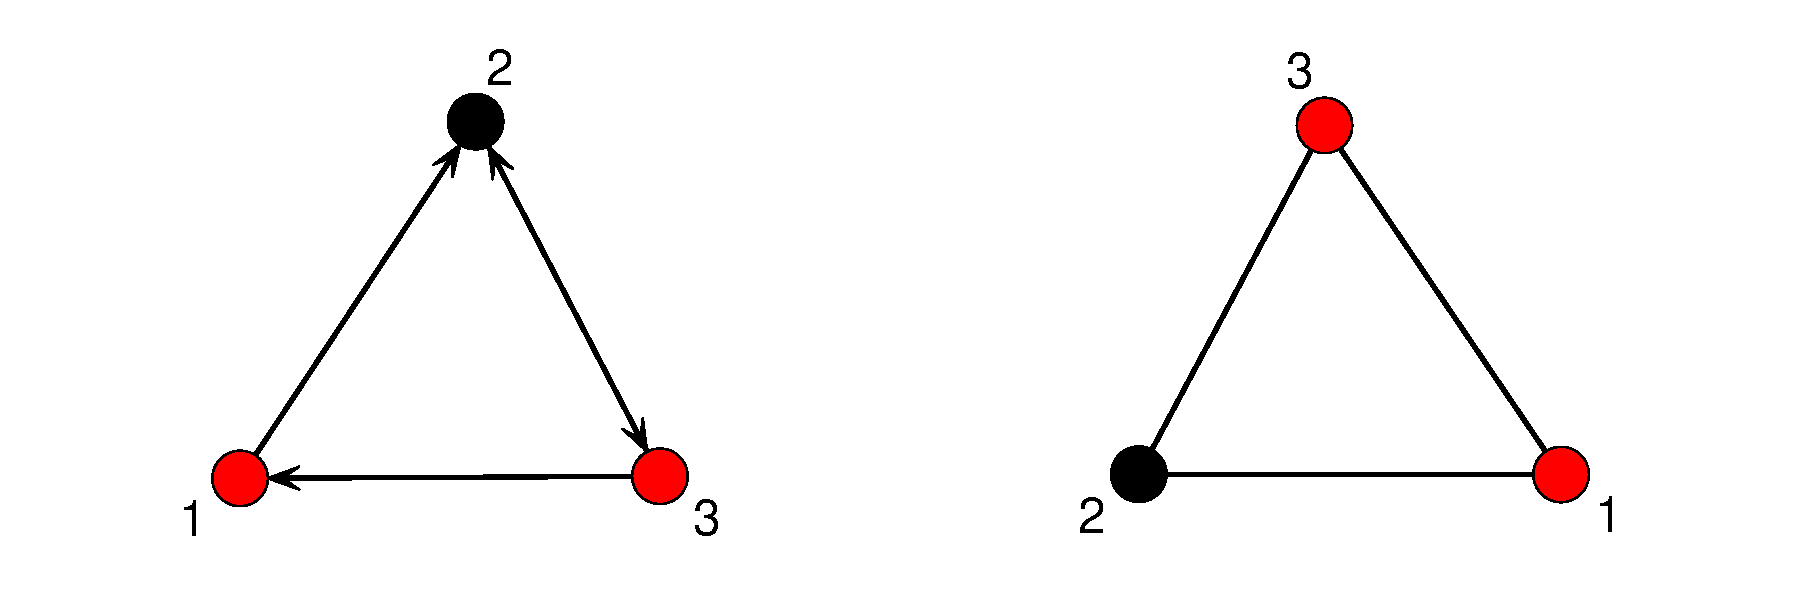
\includegraphics{paper-mininet}
\caption{A simple directed (left) and undirected (right) 3 node network}
\label{fig:mininet1}
\end{figure}

In order to be able to fit a mixed effects model on network data, we need to transform the network into an appropriate design matrix. The shape of the data
is more than an technicallity in this case. It defines what exactly we consider to be the grouping factor, which is not completely trivial. \\

For a directed graph the most straightfoward representation of the data is by completely expanding it into a matrix with one row 
for every possible edge. For example, the left network in \ref{fig:mininet1} shows an example of a tiny 3 node network,
which would be represented as listed in table \ref{minitable}. Once the data is in this form, we can use standard multilevel software
to fit a crossed effect model with a random effect on the sender and a random effect on the receiver level. 


